
\item A long circular tube of length 10 m and radius 0.3 m carries a current \( I \) along its curved surface as shown. A wire-loop of resistance 0.005 ohm and of radius 0.1 m is placed inside the tube with its axis coinciding with the axis of the tube. The current varies as \( I = I_0 \cos (300t) \) where \( I_0 \) is constant. If the magnetic moment of the loop is \( N \mu_0 I_0 \sin (300t) \), then `N` is
\begin{center}
    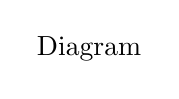
\begin{tikzpicture}
        \node at (0, 0) {Diagram}; % Replace with the actual TikZ diagram code
    \end{tikzpicture}
\end{center}
